\begin{center}

  \begin{tabular}{rp{16cm}lp{20cm}}%{rl}

  % after \\: \hline or \cline{col1-col2} \cline{col3-col4} ...

  论文地址:& \href{https://arxiv.org/pdf/2101.06861.pdf}{https://arxiv.org/pdf/2101.06861.pdf} \\
  来源:& ICLR, 2021 \\
  作者:& Chao Shang, Jie Chen, Jinbo Bi \\

  源码:& \href{https://github.com/chaoshangcs/GTS}{GTS} \\

%  slides:& \href{http://yunshengb.com/wp-content/uploads/2017/03/nips_2018_r2l_workshop_talk.pdf}{{\footnotesize Convolutional Set Matching for Graph Similarity}}\\

  关键词:& \textbf{Time series forecasting, graph
  	structure learning} \\

  写于:& \date{2021-06-15}

  \end{tabular}

\end{center}

该论文\cite{shang2021discrete}针对的是时间序列预测问题,要做到多步(multiple time)预测。论文将时间序列预测与GNN联合起来,以$T$步长的历史数据预测未来$\tau$步。

\paragraph{问题定义}
$\widehat{X}_{t+T+1: t+T+\tau}=f\left(A, w, X_{t+1: t+T}\right)$
其中$X$是时间序列数据,$X.shape = [n\_series, steps, feature]$。$X_t$表示所有时间序列在$step=t$时的特征。现有的一些论文表明利用样本之间的关系能够辅助时间序列预测。因此,论文中引入了Graph,来表示时间序列样本之间的关系。重点是如何生成这样的一个graph。


\paragraph{GTS思路}
\begin{figure}[h]
	\centering
	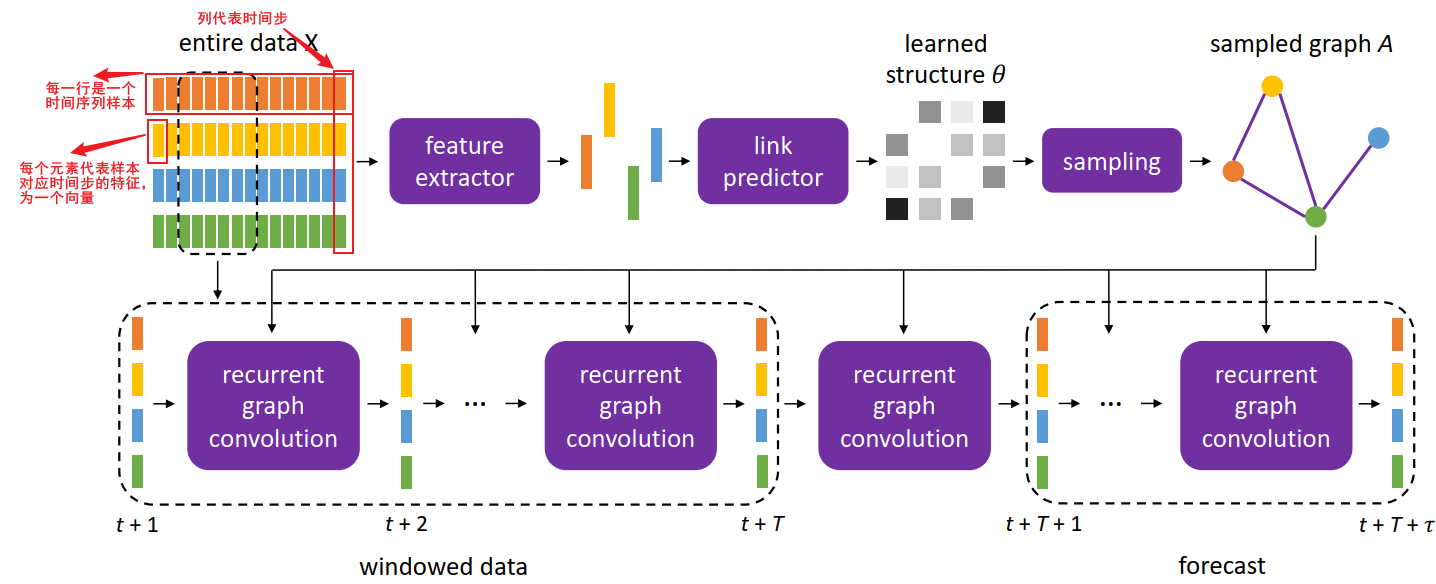
\includegraphics[width=.9\textwidth]{pics/gts.png}
	\caption{GTS Architecture}
	\label{fig:gts}
\end{figure}
GTS(Graph for time series)框架如Fig.\ref{fig:gts}所示。
看一眼损失函数:
$$
\sum_{t} \ell\left(f\left(A, w, X_{t+1: t+T}\right), X_{t+T+1: t+T+\tau}\right)
$$
很明显,在训练过程中,类似于用滑动窗口在时间序列样本的时间方向上滑动,再计算损失。具体的计算公式不用纠结。上文中提到了,要构建一个graph,那怎么构建呢?

对于n个训练样本,可以构建一个n个结点的graph,剩下的就是邻接矩阵了。论文中将邻接矩阵中每个元素(论文中构建的是有向图)的取值服从于一个伯努利分布$\theta$。$\theta$也是训练过程中学习得参数,因为邻接矩阵是从$\theta$中采样出来的,因此文中使用了Gumbel\cite{jang2017categorical}重参数化技术。模型的前向过程从Fig.\ref{fig:gts}可以体现。

\paragraph{总结}
从模型的输入可以看出,模型针对的数据主要是样本数不变的场景,如交通预测中,而且每个样本的序列长度是一致的。可以看作是针对一个固定结点集的graph,预测其结点特征。可以看作是一个回归任务,文中使用的也是均方误差作为损失。
